
%(BEGIN_QUESTION)
% Copyright 2011, Tony R. Kuphaldt, released under the Creative Commons Attribution License (v 1.0)
% This means you may do almost anything with this work of mine, so long as you give me proper credit

Suppose a pair of split-ranged control valves are used to cool hot product liquid through a heat exchanger.  Cooling water flows from a utility water header (constant pressure of 80 PSI) through the tube side of a shell-and-tube heat exchanger, while product flow may be throttled through the shell side:

$$\includegraphics[width=15.5cm]{i03409x01.eps}$$

The sequenced valve control strategy needs to work like this: first, the product valve (TV-24b) needs to remain wide-open if possible to allow maximum production flow rate, temperature control being done by modulating the flow of cooling water to the heat exchanger.  However, if even a wide-open cooling water valve (TV-24a) is not enough to maintain the product temperature at setpoint, the product valve must begin to pinch off the flow to maintain temperature at setpoint.

The only thing you are told about these two valves is that the process valve (TV-24b) is fail-open.

\vskip 10pt

Determine the proper split-range sequencing for these two valves, assuming they both operate on the same 4-20 mA analog signal from the temperature controller's output.  Assuming a standard direct-acting calibration (4-20 mA = 3-15 PSI) for the I/P transducer.  

\vskip 10pt

Also, determine the necessary action for the controller, assuming a direct-acting response from the temperature transmitter.

\vfil 

\underbar{file i03409}
\eject
%(END_QUESTION)





%(BEGIN_ANSWER)

This is a graded question -- no answers or hints given!

%(END_ANSWER)





%(BEGIN_NOTES)

The split-ranged sequencing required for this application is a kind of weird hybrid of complementary and progressive.  We need the cooling water valve to open up with increasing signal, but when that valve has reached maximum (wide-open) we need the product valve to start pinching off for more cooling effect (adding less heat to the system).  Thus, valve TV-24a needs to be shut at 4 mA, wide-open at 12 mA, and remain wide-open up to 20 mA.  The product valve TV-24b needs to be wide-open from 4 to 12 mA (for maximum production), and then pinch off from 12 mA to 20 mA:

$$\includegraphics[width=15.5cm]{i03409x02.eps}$$

The controller must be {\bf direct-acting}.

%INDEX% Final Control Elements, valve: sizing
%INDEX% Process: heat exchanger temperature/flow control (generic)

%(END_NOTES)


